\section{Introduction}

\begin{definition}[\textit{Identification}]
    Identification refers to the action where an entity declares its identifier.
\end{definition}
\begin{definition}[\textit{Authentication}]
    Authentication involves the process by which an entity provides evidence to confirm its claimed identity.
\end{definition}
Authentication can take either a unidirectional or bidirectional (mutual) form.
\begin{figure}[H]
    \centering
    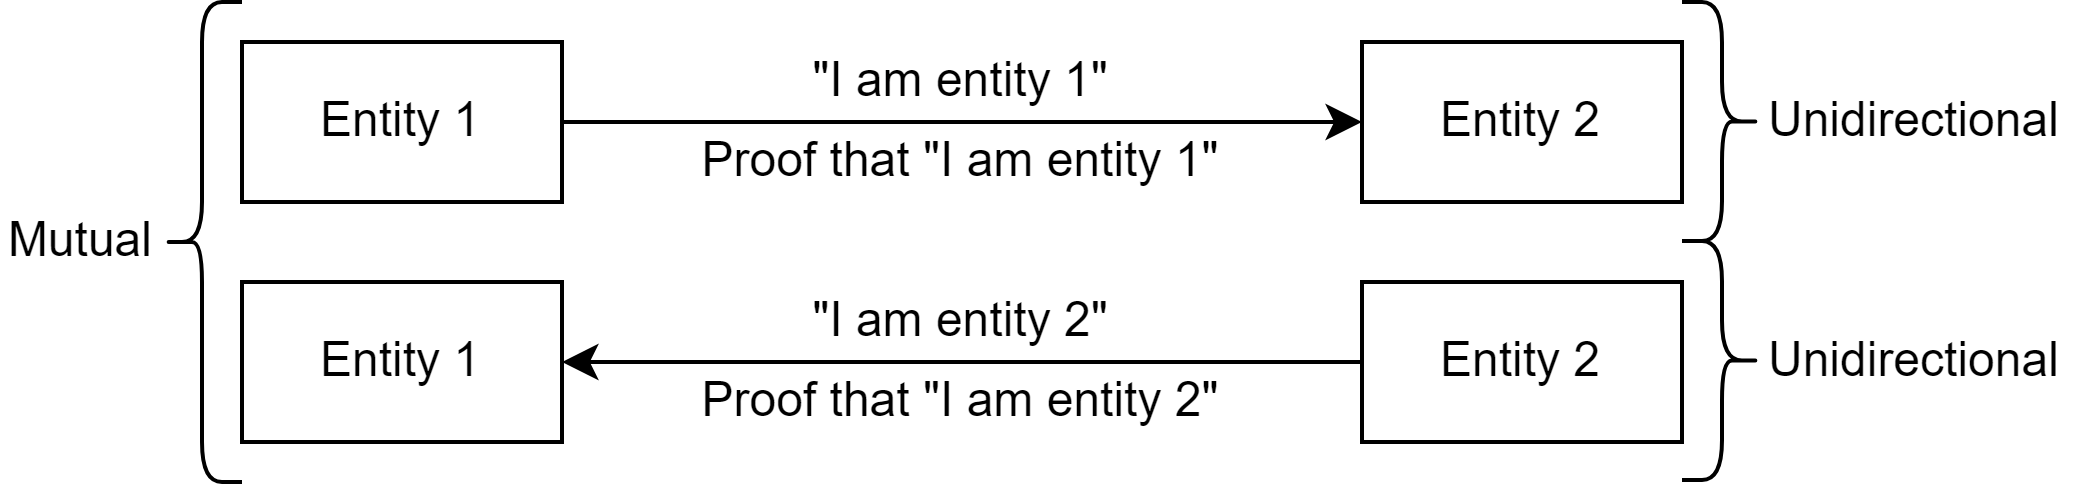
\includegraphics[width=0.75\linewidth]{images/auth.png}
    \caption{Authentication direction}
\end{figure}
This process can occur between various entities:
\begin{itemize}
    \item Human to human.
    \item Human to computer.
    \item Computer to computer.
\end{itemize}
Authentication serves as a foundational step for subsequent authorization phases.

\subsection{Factors of authentication}
Authentication factors may include:
\begin{enumerate}
    \item \textit{Knowledge-based factors}: information that the entity knows (e.g., password or PIN).
    \item \textit{Possession-based factors}: items that the entity possesses (e.g., door key or smart card).
    \item \textit{Inherent factors}: characteristics that are unique to the entity (e.g., face or voice).
\end{enumerate}
Multifactor authentication typically involves the use of two or three of these factors.

In human-centric scenarios, inherent factors are more commonly utilized than possession-based factors, and possession-based factors are more commonly used than knowledge-based factors.
In machine-centric scenarios, knowledge-based factors are more frequently employed than possession-based factors, and possession-based factors are more commonly used than inherent factors.